%\chapter{EMS}
\section{Environment Characterization Study}
\label{sect:prediction}
Another part of the research project is to look at the characteristics of the operating environment to see if it is possible to make useful (probabilistic) predictions of the evolution of those characteristics.

Whilst dynamic despatch scheduling (DDS) is recognized as a suitable technique for allocating jobs in a changing and uncertain environment \cite{cicirello01random}, it can however suffer from \emph{myopism}. Decisions are made for the current instant and typically take no consideration as to what is to happen next or over the medium or longer term horizons. Even when some consideration is made of likely future decisions or potential decisions a DDS does not generally have a way of remembering what those decisions would have been at future times. (This needs better explanation) 

Basically what this means is:- scoring ahead several groups while making \emph{best guess} assumptions about the probability of being able to execute these future groups. Game-theory describes this as the \emph{expected utility} \cite{vonneumann44games} and uses the concept of {\bf discounted future reward} to provide a mechanism for integrating a probabilistic element into the look-ahead.  Namely that potential rewards which may be received in the future are worth \emph{less} compared to rewards received immediately. 

\subsection{What - Operating Environment}
As has already been stated (somewhere in intro chapter)- the telescope operates in an uncertain environment - various sources of uncertainty can lead to periods of downtime where the telescope is unavailable. These can be roughly broken down into the categories of technical, weather and sky conditions.

\begin{description}
\item [technical] Failure or deliberate (preventative maintainance) shutdown of mechanical, electrical, software or communications systems can leave the telescope non-operational.
\item [weather] Bad weather forces the shutdown of the telescope systems to prevent damage. Typical examples include:- closure due to rain to prevent ingress of water into delicate instrument, optical and electrical hardware; closure due to high humidity to prevent condensation on optical and electrical hardware; closure due to high or gusting winds both to protect mechanical structure and due to reduced tracking from wind-shake; calima (Saharan dust) a problem during the summer months forces closure to prevent damage to optical and mechanical systems.
\item [sky conditions] Poor sky conditions do not pose problems for infrastructure but can severely disrupt the ability to perfom useful observations:- extremly bad seeing, high extinction forces long exposures to achieve required SNR, similarly for high sky brightness.
\end{description}
  
Many of these processes are naturally unpredictable, however it would be very useful to be able to at least have some way to determine likeliness of these conditions occurring.


\subsection{why}
Why is this needed - discussion notes elsewhere plus stuff on LAS and expected utility. (pull these next 2 blocks together)

This is important for a number of reasons:-
\begin{itemize}
\item In order to schedule OGs at a future time which is both suitable and ideally optimal it is neccessary to be able to determine the likelihood of actually performing the observations at such times.
\item To determine the likeliness of particular conditions at future times (in terms of condition matching).
\item To incorporate future availability into medium / long term plans.
\item To be able to predict execution probability accurately on behalf of external agents.
\end{itemize}

Discuss differing timescales.
\begin{itemize}
\item a Current scheduling horizon - typically of the order hours.
\item b Current scheduling night.
\item c Next few nights upto one week.
\item d Next few weeks.
\item e Current semester.
\end{itemize}

Discuss some examples i.e.likely use cases/scenarios).
\begin{itemize}
\item a Should I execute group X now followed by Y or execute Y now which is more profitable and expect to do X in about an hour when it is more profitable thus achieving maximum profit.
\item b Can I postpone critical group X for now and expect to do it later tonight when its less busy.
\item c If I postpone non-critical group X until tomorrow soas to execute critical group Y tonight what are the chances I will get X done.
\item d What fraction of the executions (yield) of monitoring group X am I likely to achieve over the next few weeks.
\item e How will the likely split of resources compare to TAG allocated targets over the comming semester.
\end{itemize}

% ------------------------
% REVIEW OF PREVIOUS WORK
% ------------------------
\subsection{Background/review of previous work on site character (not prediction)}
Collect data from various sources - SQG papers and web stuff.

NAO - negative correlation with January precipitation - cyclic phenomenon - predictable? (Refs)

Presence of inversion layer (600-1000m) means different weather characteristcis from sea-level.

Night-sky emission spectrum (Benn and Ellison lapalma TN).

Review of present research and statistics -climatology.

\subsubsection{Meteorology}
Meteorological data has been collected on the ORM site for xxx years, in particular the largest and most comprehensive set of continuous meteorological station readings going back to 1985 have been recorded by the Isaac Newton Group (ING). Other telescopes on the site have meteorological data covering lesser periods. 

The ORM site is at 2400m near the summit of the Roche de los Muchachos just North of the rim of the caldera de Taburente. 

The ING annual report 2000-2001 gives details of weather downtime for the ING telescopes of around 20\% per year. The data for period 1991-2001 shows a variation between a minimum of 16\% annual loss in 1998 to a maximum of 37\% in 1996. Seasonally the minimum downtime of around 3\% occurs in summer (June,July,August) with increasing levels of downtime either side reaching a maximum of upto 40-45\% during the worst months of December and January. The 2005 annual report shows a peak of around 80\% weather loss during february 2005 - \emph{the great snow}. 


\subsubsection{Seeing}
The atmospheric seeing regime has been studied for many years both through short campaigns and as part of longer studies aimed at site testing for telescopes such as the Grande Telescopio Canarias (GTC).
 A short study in 1990 by \cite{vernin92optical} on the contributions of the various air layers above the site suggests that the main contribution, some 50\% comes from air in the boundary layer (from a few meters to 1 km above the ground. They found that 40\% is provided by the free air above 1 km and that 8\% comes from the surface layer of the first few meters. Sources internal to the dome (the NOT) provide the remaining 2\%.

A longer 9 month study \cite{munoz97nighttime} using a DIMM mounted on a 5m tower (above the surface layer) concluded that the inversion layer which lies below the observatory site is of particular importance in determining seeing characteristics. The layer generally lies between 1200m and 1500m, well below the site at 2400m and acts to suppress convection - a layer of strato-cumulus is generally seen at the top of this layer. Around 55\% of the local atmospheric humidity is trapped below the layer with around 20\% above. They find that the best seen correlates with those time when the inversion layer is at its lowest (around 1200m and strongest (largest temperature difference between top and bottom of the layer) which occurs in the summer months (June,July, August). At this time the strength of the trade winds is highest. They find that during the summer the average seeing is 0.61'' and median 0.5''. During the remaining months the average seeing is 0.77'' and median 0.91''. 

\cite{munoz97nighttime} also studied some time variation effects finding that typically seeing can change very abruptly - deteriorating within a few minutes but that it rarely returns to a stable level so quickly - typically they find a recovery time of around 2 hours - they put this down to the effects of sudden perturbations in a steady atmospheric flow giving rise to turbulence which can take some time to settle. Some oscillatory effects were recorded with a period of around 45 minutes. 

A year long study by \cite{munoz98homogeneity} on the variation of seeing between different sites at the ORM revealed an average seeing of 0.72'' and median 0.65''. They found relatively small variation between sites except when the seeing was particularly poor when the variation was more pronounced - upto 0.2'' between locations. In summer they find that seeing is better than 0.5'' for 50\% of the time dropping to 25\% averaged over the whole year. A correlation was found between wind speed and direction and seeing quality. 

At low wind speed (<5 km/h) there was no relation between wind direction and seeing. At medium wind speed (5 - 15 km/h) they found the best seeing associated with Northerly winds and poor seeing when the wind was Southerly (from over the Caldera rim). At high wind speeds (> 45km) seeing was generally very poor). 

\subsubsection{Extinction}
A study of the contributions to extinction at the ORM was made by \cite{lapalma31}. This gives formulae for the calculation of the contributions from rayleigh scattering and absorption by ozone and water-vapor. They find that the contribution from ozone can vary significantly during the year and even on timescales of a few hours.

A major contribution to extinction is the dust (calima) contained in the Saharan Air Layer (SAL). This dust is thrown up from the Saharan desert by predominatly South Easterly winds and the pushed West over the Canaries and Atlantic often reaching as far as South America and the Caribbean. In a study comparing CAMC extinction measurments with data derived from satellites \cite{varelo07sat} find that during summer around 75\% of nights are dust-free but during the rest of the year this rises to around 90\%. Episodes of calima can however occur sporadically at other times. They find that $k_V$ is typically $< 0.2 mag/airmass$ for 88\% of times and $> 0.5 mag/air,ass$ for 1\% of nights with a modal value of 0.11.

A study of 2850 nights of CAMC data by \cite{guerrero98diurnal} reveals that most dust is present during June to September (coincidentaly the period of best seeing), they also note large changes in mean extinction during 1991 and 1982 corresponding to eruptions of Mt. Pinatubo and El Chichon.

\subsubsection{Sky brightness}
The sky background is composed of contributions from (in decreasing order of precedence):-
\begin{itemize}
\item Airglow - 
\item Zodiacal light -
\item Starlight -
\item Stars ($V > 20$) -
\item Extragalactic light -
\item Light pollution -
\end{itemize}
Need some explanations for those (see ING TN-115).

A detailed description and estimates are given by \cite{lapalma115}. They find the relative contribution from airglow and zodiacal light to be around 2.5:1 at high ecliptic latitude while at lower latitude the sky is brighter by 0.4 mag. The mean brightness across the sky does not vary by more than 0.1 mag between times of astronomical twilight. They present a formula for calculation of the sky brightness in V as a function of sky position in moonless conditions. A detailed study of the sky-brightness under moonlight conditions is presented in \cite{krisciunas91brightness}. 



% TECH DOWNTIME
\subsection{Technical downtime}
The nature of the problem...

Periods where observing has been disrupted due to technical problems. These can be caused by a number of different systems and can be roughly classified into:-

\begin{description}
\item [Mechanical] Physical problems with mechanical components such as:- main axes, focus drive, enclosure hydraulics, science fold deployment and instrument components such as filter-wheels.
\item [Electrical] Power supplies to the site are occasionally disrupted, often this information is available in advance.
\item [Network] Problems due to internal (inter-system) communications breakdown - maybe as simple as a wire dropped out, a software configuration problem or due to heavy network loading - typically a symptom of some other underlying problem. Often fixed on the same day. 
\item [Software] Low and high level systems can cause problems. These are highly complex systems and thus difficult to test thouroghly even with use of simulated environment so problems often occur during upgrades. 
\item [Other]
\end{description}

From general knowledge of the operating procedure it is clear that technical problems follow a variety of timelines (workflows) and we can classify these into a few basic categories:-
\begin{description}
\item [\emph{major catastrophy}] These are problems which suddenly manifest themselves one night causing major downtime. Typically these are due to either mechanical breakdown of a component which requires a site visit to repair - the time involved can potentially be days if spares are not immediately available and no workround can be arranged or are due to major software failure - these tend to involve a major software effort the following day and are generally fixed within the day. 
\item [\emph{occasional glitch}] These are problems due to either non-terminal failure of a mechanical component which is too expensive to justify replacing or more often a known but difficult to repair software problem. The frequency of occurance will tend to determine how much effort is used on the solution.
\item [\emph{sporadic bug}] Sometimes the problem is very difficult to identify and needs to occur many times before enough information is gathered to identify the cause. 
\item [\emph{shakedown}] Effectively time required for new mechanical components or software deployments to bed in. Software in particualr may be tested on the simulator but behave differently on the actual system due to subtle timing effects or unpredicted coincident situations.
\end{description}


\subsubsection{Source of data}
The main source for this information is the nightly logs kept by telescope operations staff. These consist of the number of hours of technical downtime, weather downtime and actual observing hours per night. This information is assessed by a combination of examining system logs and from personnal knowledge of the events of the previous night and so a degree of interpretation is involved. Of particular importance is the policy to assign the category \emph{weather downtime} to those periods when there was a combination of bad weather and technical problems - it is thus not possible to seperate these out. E.g. on a night where there might be 2 hours of observing mixed with 2 hours of intermittent technical problems followed by 6 hours of bad weather there is no way of telling whether the actual technical problem would have resulted in an additional period of downtime if the weather had remained good. Operations staff may assess early in the night that some serious technical problem is likely to affect the performance of the telescope during the night - e.g. poor image quality or tracking and decide to shutsown the telescope for the remainder of the night thus yielding an apparently high loss fraction rather than allow the automated systems to cycle between \emph{operational} and \emph{impaired}.

Data covering a period of 30 months (919 days) for 2005, 2006 and part of 2007 was available and used to determine a figure for probability of technical downtime and how this varies over the year. 

\subsubsection{Analysis and Results}

Plots of technical downtime per night are displayed in Figs. (\ref{fig:nightly_tech2005},\ref{fig:nightly_tech2006} and\ref{fig:nightly_tech2007} ) 

\begin{figure}[htbp] 
\begin{center}
 
 \subfigure[Technical downtime per night 2005.] {
    \label{fig:nightly_tech2005}
    \includegraphics[scale=0.4, angle=-90]{figures/ecs/met_nightly_stats_tech2005.eps}
  }
 \subfigure[Technical downtime per night 2006.] {
    \label{fig:nightly_tech2006}
    \includegraphics[scale=0.4, angle=-90]{figures/ecs/met_nightly_stats_tech2006.eps}
  } 
 \subfigure[Technical downtime per night 2007.] {
    \label{fig:nightly_tech2007}
    \includegraphics[scale=0.4, angle=-90]{figures/ecs/met_nightly_stats_tech2007.eps}
  }
\caption{Nightly hours plots for technical downtime for years 2005,2006,2007(part). Large blocks are empty due to operations policy preference for reporting bad weather downtime rather than technical when both occur simulataneously.}
\end{center}
\label{fig:met_nightly_tech}
\end{figure}


Fig.~\ref{fig:tech_loss_dist} shows the distribution of fraction of night lost to technical problems, as can bee seen this is bimodal with around 72\% of nights suffering less than 5\% downtime (including those nights with zero loss). A total of 8\% of affected nights over the entire period suffered nearly 100\% downtime.  

\begin{figure}[htbp]  
  \begin{center}
    \includegraphics[scale=0.4, angle=-90]{figures/ecs/tech_loss_frac.eps}
  \end{center}
  \caption[Distribution of fraction of night lost to technical problems.]
   {Distribution of fraction of night lost to technical problems. Majority of nights have less than 5\% loss, while some 8\% suffer near 100\% downtime.}
  \label{fig:tech_loss_dist}
\end{figure}

The variation of total technical downtime hours averaged by month for the available data is shown in Fig.~\ref{fig:monthly_tech_stats}. The average monthly downtime is 11.94 hrs over the period corresponding to about 0.46 hours per night.

\begin{figure}[htbp]
  \begin{center}
    \includegraphics[scale=0.4, angle=-90]{figures/ecs/monthly_tech_stats.eps}
  \end{center}   
  \caption[Monthly averaged technical downtime hours.]
{Monthly averaged technical downtime hours over the period 2005-2007 (30 months). The data only includes periods where there was no weather downtime. Average time per month lost 11.94 hrs or 0.46 hours per night}
  \label{fig:monthly_tech_stats}
\end{figure}


\subsubsection{Conclusions}
It had been hoped to look at lengths of runs of technical downtime to determine if there were any patterns - e.g. do these occur in runs and what is the length distribution and frequency of these. Contamination of the data from weather downtime stats and the relatively small amount of data available makes this problematic. Heuristically however we might expect this to be the case - a problem arises sporadically one night, maybe occurs the following night and spawns attempts by support staff to solve by software or engineering means. This may occur quickly or take several nights to correct, thereafter the problem disappears or becomes less frequent.

The diverse nature of these problems suggests that there is little chance of predicting future occurances - by their very nature they are unpredictable - the best that can realistically be achieved is to use the long term probabilities to estimate the likelihood of technical downtime over extended periods. 

Disruption to power supplies are sometimes known in advance and could be factored into the scheduler. Periods of planned maintainance are often known well in advance and could also be factored in - infact both these are implicitly taken account of by the operations team when setting up the content of the phase2 ODB but this information is not currently known explicitly by the scheduler - this will become more important when users are able to update their own phase2 information.

Any more comments here...

% WEATHER
\subsection{Weather}
Weather data has been obtained from 2 independant sources.
\begin{itemize}
\item The LT's own weather monitoring system (WMS). WMS data has been collected by embedded software for a period of 20 months/583 days at a cadence of approximately once every 32 seconds with very few gaps giving a total of 1582518 samples (see gap distribution histogram in Fig. \ref{fig:gap_dist} ).
\item Archived met station data from the various facilities at the ORM are available (XXX refs).
\item Observer reports of weather downtime hours per night (collated next day) for reporting on the telescope website. This data is bundled in with the technical downtime statistics and overrides these when both occur on the same night.
\end{itemize}


\subsubsection{Telescope Weather Monitoring System}
 The Weather Monitoring System (WMS) provides feeds of various meteorological data from a weather station on site located XXXm from the telescope enclosure. (some basic info about the thing like who built it etc). Data is provided to the RCS at a cadence of around 5 seconds. The RCS filters this data and uses a set of rules (Table. \ref{tab:rcs_weather_rules}) to decide if the weather should be classified as \emph{good} in which case (all things being otherwise okay) observing may proceed, or \emph{bad} in which case observing may not proceed or if already underway should be stopped and the telescope and enclosure made safe.

Weather shutdowns based on WMS data are triggered by any of the following sources:-
\begin{itemize}
\item High humidity can lead to condensation on cold surfaces (mirror, electricals) and is an indicator of cloud and potential precipitation.
\item Rain causes wetting of all equipment, this has to be avoided especially on sensitive optical, electrical and hydraulic systems.
\item Moisture fraction is indicated by a digital sensor and indicates that rain or condensation is occuring or has recently occurred but not yet cleared sufficiently.
\item Cold temperatures lead to ice which can cause the enclosure portals to stick and thus put considerable strain on the motors and electrical supply if an attempt was made to open these.
\item Wind gusts  can cause damage to telescope structure and attached instruments. Moderate wind can also lead to poor tracking performance due to \emph{wind shake}.
\end{itemize}

Table \ref{tab:rcs_weather_rules}) summarizes the rules currently (January 2008) in force for weather clear and alert triggers. A weather variable crossing its \emph{alert} level signals bad weather. In order to clear (signal good weather) the variable must pass the primary \emph{clear} level and remain below the secondary level for at least the time specified by the stability parameter. All variables must be in the \emph{clear} state for overall {\bf Good} weather. Any variable in its \emph{alert} state indicates {\bf bad} weather. Currently all rules have a 30 minute clearing stability time but this can be changed.

\begin{table}[htbp]
\begin{center}
\begin{tabular}{lllll}
\toprule
\multicolumn{5}{c}{Weather variable triggering conditions} \\
\midrule
Variable & Alert threshold & Primary clear level & Secondary clear level & Stability \\
\midrule
Humidity    &  $> 80$\%        & $< 70$\%         & $< 75$\%          & 30 min\\
Moisture    &  $> 10$\%        & $< 9$\%          & $< 9.5$\%         & 30 min\\
Wind speed  &  $> 15ms^{-1}$   & $< 12ms^{-1}$    & $< 14ms^{-1}$     & 30 min\\
Temperature &  $< 0.0^{\circ}$ & $> 0.1^{\circ}$C & $> 0.05^{\circ}$C & 30 min\\
\bottomrule
\end{tabular}
\end{center}
\caption{Definitions of alert and clear threshold levels for triggering good/bad weather conditions. A variable crossing its alert level signals bad weather. In order to clear (signal good weather) the variable must pass the primary clear level and remain below secondary level for at least the time specified by stability parameter. All variables must be in the \emph{clear} state for overall {\bf Good} weather. Any variable in its \emph{alert} state indicates {\bf bad} weather.}
\label{tab:rcs_weather_rules}
\end{table}

The data collected consists of 1582518 samples taken at around 30 seconds cadence over a period of 30 months between 2005 and 2007. The inter-sample gap distribution (Fig.~\ref{fig:gap_dist}) shows relatively few gaps. 364 gaps exceed 5 minutes of which 58 also exceed 60 minutes. The longest gap of 4.2 days occurred on XXX due to a power outage.  
\begin{figure}[htbp]
  \begin{center}
    \includegraphics[scale=0.4, angle=-90]{figures/ecs/gap_dist.eps}
  \end{center}
  \caption[Distribution of intersample gaps.]
{Distribution of intersample gaps. The vast majority of the 1582518 samples occur with gaps of 30 seconds. A small number 292 excede 5 minutes, a further 14 excede 30 minutes and 58 excede 60 minutes. The largest gap of 4.2 days occurred during xxx as a result of a site power outage.}
  \label{fig:gap_dist}
\end{figure}


\subsubsection{Analysis of results}
Look specifically at humidity data - this is generally the deciding factor in weather shutdowns.

The distribution of humidity is shown in Fig.~\ref{fig:met_humidity_dist}.  A cumulative distribution is shown in Fig. \ref{fig:met_humidity_cum_dist}. The distributions show an approximately normal profile with a peak around 15\% and average of \%. A very sharp secondary peak occurs around 95-100\% humidity. With the variable trigger levels (\ref{tab:rcs_weather_rules}) set to 70\% (\emph{clear}) and 80\% (\emph{alert}) these can both be seen to be well into the tail of the normal distribution just before the spike. This suggests that few false alerts should occur.

\clearpage 
\begin{figure}[htbp]
  \begin{center}
    \includegraphics[scale=0.4, angle=-90]{figures/ecs/hum.dat.eps}
  \end{center}
  \caption[Relative distribution of humidity at telescope site.]
{Distribution of atmospheric humidity at the telescope site over all samples. The distribution shows a normal profile with peak around 15\% and average of \%. A very sharp secondary peak occurs around 95-100\% humidity. With the variable trigger levels set to 70\% good and 80\% bad these are in the tail of the normal distribution just before the spike level...}
  \label{fig:met_humidity_dist}
\end{figure}
\begin{figure}[htbp]
\begin{center}
    \includegraphics[scale=0.4, angle=-90]{figures/ecs/hum_cum.dat.eps}
\end{center} 
\caption[Cumulative distribution of humidity at telescope site.]
{Cumulative distribution of atmospheric humidity at the telescope site over all samples.}
\label{fig:met_humidity_cum_dist}
\end{figure}

% Moisture fraction
\clearpage 
\begin{figure}[htbp]
\begin{center}
     \includegraphics[scale=0.4, angle=-90]{figures/ecs/moist.dat.eps}
\caption[Relative distribution of moisture fraction at telescope site.]
{Relative distribution of moisture fraction at telescope site.}
\end{center}   
\label{fig:met_moisture_dist}
\end{figure}

\begin{figure}[htbp]
\begin{center}
    \includegraphics[scale=0.4, angle=-90]{figures/ecs/moist_cum.dat.eps}
\caption[Cumulative distribution of moisture fraction at telescope site.]
{Cumulative distribution of moisture fraction at telescope site.}
\end{center} 
  \label{fig:met_moisture_cum_dist}
\end{figure}

% Wind speed
\clearpage 
\begin{figure}[htbp]
\begin{center}
    \includegraphics[scale=0.4, angle=-90]{figures/ecs/ws_25.dat.eps}
\caption[Relative distribution of wind speed at telescope site.]
{Relative distribution of wind speed at telescope site.}
\end{center} 
  \label{fig:met_windspeed_dist}
\end{figure}

\begin{figure}[htbp]
\begin{center}
    \includegraphics[scale=0.4, angle=-90]{figures/ecs/ws_25_cum.dat.eps}
\caption[Cumulative distribution of wind speed at telescope site.]
{Cumulative distribution of wind speed at telescope site.}
\end{center} 
 \label{fig:met_windspeed_cum_dist}
\end{figure}

% Temperature
\clearpage 
\begin{figure}[htbp]
\begin{center}
    \includegraphics[scale=0.4, angle=-90]{figures/ecs/temp_1525.dat.eps}
\caption[Relative distribution of temperature at telescope site.]
{Relative distribution of temperature at telescope site.}
\end{center}   
 \label{fig:met_temp_dist}
\end{figure}

\begin{figure}[htbp]
\begin{center}
    \includegraphics[scale=0.4, angle=-90]{figures/ecs/temp_1525_cum.dat.eps}
\caption[Cumulative distribution of temperature at telescope site.]
{Cumulative distribution of temperature at telescope site.}
\end{center}
    \label{fig:met_temp_cum_dist}
\end{figure}

Results (Table~\ref{tab:comp_meteo_trigs})show that humidity is greatest contributor to bad weather, consequently it is reasonable to use this alone for any prediction studies.
\begin{table}[htbp]
\begin{center}
\begin{tabular}{ll}
\toprule
\multicolumn{2}{c}{Fraction of weather variable above alert trigger level} \\
\midrule
Variable & Fraction above alert level\\
\midrule
Humidity    & 18\%  \\
Moisture    & 10\%  \\
Wind speed  & 2\%   \\
Temperature & 3.7\% \\
\bottomrule
\end{tabular}
\end{center}
\caption[Fraction of recorded weather variable statistics over \emph{alert} level.]{Fraction of recorded weather variable statistics over \emph{aler} level. Humidity is the largest contributor at 18\%.}
\label{tab:comp_meteo_trigs}
\end{table}


Based on humidity data, Fig. \ref{fig:wms_hum_frac_time} shows relative fraction of \emph{good} weather over various sized time bins. bearing in mind the small period of data available (in climatological sense) there appears to be a tendency for better weather in summer (May-July) with increasingly higher fraction of bad weather in winter in accord with general observations.

\begin{figure}[htbp]
\begin{center}
    \includegraphics[scale=0.4, angle=-90]{figures/ecs/hum_frac_time.eps}
\end{center} 
\caption[Monthly averaged good weather fraction ($1-\Delta_W$) based on humidity level.]
{Monthly averaged good weather fraction ($1-\Delta_W$) over the period 2005-2007 (20 months) based on WMS humidity levels averaged with various bin sizes.} 
\label{fig:wms_hum_frac_time}
\end{figure}


The lengths of periods of continuously good and bad weather based on the humidity triggering rule and stability settings are shown in Fig. \ref{fig:good_bad_hum_dist}. A rapid drop off suggests that long periods of continuous good/bad weather are rare, however outliers make this awkward as source for prediction.

Some examples of individual nights with particular humidity profiles.

\clearpage
\begin{figure}[htbp]
\begin{center}
  \subfigure[Humidity profile 2007-01-29.] {
    \label{fig:hum_profile_2007_01_29}
    \includegraphics[scale=0.25, angle=-90]{figures/ecs/hum_1_2007_01_29.eps}
  }
  \subfigure[Humidity profile 2007-02-20.] {
    \label{fig:hum_profile_2007_02_20}
    \includegraphics[scale=0.25, angle=-90]{figures/ecs/hum_1_2007_02_20.eps}
  }
 \subfigure[Humidity profile 2007-03-26.] {
    \label{fig:hum_profile_2007_03_26}
    \includegraphics[scale=0.25, angle=-90]{figures/ecs/hum_1_2007_03_26.eps}
  }
 \subfigure[Humidity profile 2007-03-28.] {
    \label{fig:hum_profile_2007_03_28}
    \includegraphics[scale=0.25, angle=-90]{figures/ecs/hum_1_2007_03_28.eps}
  }
 \subfigure[Humidity profile 2007-04-15.] {
    \label{fig:hum_profile_2007_04_15}
    \includegraphics[scale=0.25, angle=-90]{figures/ecs/hum_1_2007_04_15.eps}
  }
 \subfigure[Humidity profile 2007-04-16.] {
    \label{fig:hum_profile_2007_04_16}
    \includegraphics[scale=0.25, angle=-90]{figures/ecs/hum_1_2007_04_16.eps}
  }
\end{center}  
\caption{Example humidity profiles.}
\label{fig:humidity_profile_examples}
\end{figure}

Look at ratio of lengths of consecutive good/bad periods Fig. \ref{fig:met_hum_gbc} TBD TBD.

Idea behind these is something like: If we are $x$ hours into a period of good humidity then based on the known distribution of lengths the end of that period is approaching and the probability of this occurring in the next $y$ hours is given by integrating the PDF appropriately from $t=x$ to $t=y$. This will on average give the correct probability but for subsequent days we may do just as well using climatological statistics.

XXX Look at periodicity - Lomb periodogram. (not likely)

\subsubsection{Conclusions/prediction}
Several models for simple prediction have been tested to determine which if any provide good results.

Without additional information the best we can do is to use the long-term climatological prediction. Based on the data plotted in Fig. {\ref{fig:good_bad_period_time} showing the lengths of periods of continuous \emph{good} and \emph{bad} weather it was found that approximately  80.35\% of all time constitutes \emph{good} weather and the remainder (19.65\%) is \emph{bad} weather.

The first model (M1) is based on the assumption that the weather will continue in its current state for a period roughly equal to the length of time it has already been in that state continuously, thereafter the probability of maintaining this state decreases, assumed exponentially with a decay length some multiple of the current stability period. As an example, assume the weather has been \emph{good} for about 3 hours. We then assume it will continue to remain \emph{good} for about another 3 hours with the probability decaying as $exp{-t/3m}$ - the 3 being the amount of time already in this state, $m$ being a scale factor yet to be determined. Fig. \ref{fig:good_bad_hum_dist} shows the variation of lengths of consecutive periods of good and bad weather based on humidity threshold (80\% trigger) and clearing stability time of 30 minutes. We see that shorter periods are most common with the average length of \emph{good} periods being 31.5 hours and bad periods being 7.7 hours. Cumulative plots are shown in Fig. \ref{fig:good_bad_cumhum_dist}. The overall fraction of time classified as \emph{good} resulted in 80.35\% of all time with \emph{bad} weather making up the remainder.

\begin{figure}[htbp] 
\begin{center}
    \includegraphics[scale=0.4, angle=-90]{figures/ecs/good_bad_hum_bin.eps}
\end{center}
\caption[Cumulative probability of lengths of good/bad weather runs.]
{Cumulative probability of lengths of good/bad weather runs.}
\label{fig:good_bad_hum_dist}
\end{figure}

\begin{figure}[htbp] 
\begin{center}
    \includegraphics[scale=0.4, angle=-90]{figures/ecs/good_bad_cumhum_bin.eps}
\end{center}
\caption[Cumulative probability of lengths of good/bad weather runs.]
{Cumulative probability of lengths of good/bad weather runs.}
\label{fig:good_bad_cumhum_dist}
\end{figure}

A set of simulations were run using the extracted period data (Fig. {\ref{fig:good_bad_period_time}) to determine the effectiveness of this prediction mechanism. Every 15 minutes through the available period a determination is made of the current weather state and how long ($\tau_G$ \emph{good}) or ($\tau_B$ \emph{bad}) it has been in that state. A prediction is made at a number steps into the future (192 steps of 15 minutes constituting upto 48 hours look-ahead) using the rule specified in Eqn.\ref{eqn:prediction_decay}. At each step the prediction is compared to the actual weather state at the time and counted as either a hit (correct prediction) or miss (incorrect prediction). The final percentages shown in Fig. \ref{fig:gbc_prediction} against look-ahead time for a number of decay scale factors $m$. The baseline of 80.35\% represents the worst we should be able to acheive on average based on long-term climatological prediction - basically if we always just guess that the weather will be good this will work 80.35\% of the time. Fig. \ref{fig:gbc_m_crossover} shows the crossover point - the length of look-ahead where the prediction becomes worse than long-term climatological prediction as a function of the decay scale factor $m$. This is seen to converge towards a value of 30-31 hours which is close to the average length of \emph{good} weather period.

\begin{equation}
\label{eqn:prediction_decay}
P_{good}(\Delta T) = 
\begin{cases} 
\Delta T < \tau_G : & 1   \\ 
\Delta T > \tau_G, \tau_G < T_G : & e^{\frac{\Delta T-\tau_G}{m \tau_G}} \\
\Delta T > tau_G , \tau_G > T_G : & e^{\frac{\Delta T-T_G}{m \tau_G-T_G}}
\end{cases}
\end{equation}


\begin{figure}[htbp]
\begin{center}
    \includegraphics[scale=0.4, angle=-90]{figures/ecs/gbc_period.eps}
\end{center}
\caption[Time variation of lengths of good/bad periods based on humidity level.]
{Time variation of lengths of good/bad periods based on humidity level.}
\label{fig:good_bad_period_time}
\end{figure}


\begin{figure}[htbp] 
  \begin{center}
    \includegraphics[scale=0.4, angle=-90]{figures/ecs/gbc_predict.eps}
  \end{center}
  \caption[Accuracy of look-ahead weather prediction using time decay model against look-ahead time]
  {Effect of time scaling-factor (m) on variation of prediction accuracy of time decay prediction model against look-ahead time. All plots show a decay with time. As the scale factor is increased the cross-over point for the prediction against climatological baseline prediction of 80.03\% approaches a maximum of around 31 hours. }
  \label{fig:gbc_prediction}
\end{figure}

\begin{figure}[htbp]
  \begin{center}
    \includegraphics[scale=0.4, angle=-90]{figures/ecs/m_crossover.eps}
  \end{center}   
  \caption[Variation of cross-over point for look-ahead weather prediction using time decay model with scale factor.]
  {Variation of cross-over point for look-ahead weather prediction using time decay model with scale factor. The crossover point is seen on converge on a value around 30-31 hours which corresponds closely to the average length of good weather periods (31.5 hours).}
  \label{fig:gbc_m_crossover}
\end{figure}



% some graphs showing the data for 2005 2006 2007 

\subsubsection{Observer reports}
The observer-reported hours-per-night data for weather downtime are displayed in figures \ref{fig:nightly_weather2005} for 2005 , \ref{fig:nightly_weathe2006} for 2006  and\ref{fig:nightly_weathe2007} for 2007 (part).

Figure (\ref{fig:ecs_monthly_weather_stats}) shows the variation of weather downtime fraction, the fraction of the potential obseerving hours per night lost to bad weather ($\Delta_W$) averaged by month for the available data. June is the best month with less than 10\% of potential observing time lost to weather. February is worst with 58\% of potential observing time lost to weather.

\begin{figure}[htbp]
\begin{center}
    \includegraphics[scale=0.4, angle=-90]{figures/ecs/monthly_weather_stats.eps}
\end{center}   
\caption[Monthly averaged weather downtime fraction.]
{Monthly averaged weather downtime fraction over the period 2005-2007 (30 months). There is a relatively smooth variation between summer and winter figures with typically less than 10\% loss in June (best month) and upto 58\% loss in February (worst).}
 \label{fig:ecs_monthly_weather_stats}
\end{figure}


%\clearpage
\begin{figure}[htbp]
\begin{center}
 \subfigure[Weather downtime per night 2005.] {
    \label{fig:nightly_weather2005}
    \includegraphics[scale=0.4, angle=-90]{figures/ecs/met_nightly_stats_weather2005.eps}
  }
 \subfigure[Weather downtime per night 2006.] {
    \label{fig:nightly_weather2005}
    \includegraphics[scale=0.4, angle=-90]{figures/ecs/met_nightly_stats_weather2006.eps}
  } 
 \subfigure[Weather downtime per night 2007.] {
    \label{fig:nightly_weather2005}
    \includegraphics[scale=0.4, angle=-90]{figures/ecs/met_nightly_stats_weather2007.eps}
  }
\end{center}
\caption{Nightly hours plots for bad weather for years 2005, 2006, 2007(part)}  
\label{fig:met_nightly_weather}
\end{figure}

And the observing hours per night are displayed in figures \ref{fig:nightly_obs2005} for 2005 , \ref{fig:nightly_obs2006} for 2006  and\ref{fig:nightly_obs2007} for 2007 (part)..

%\clearpage
\begin{figure}[htbp]
\begin{center}
 \subfigure[Observing hours per night 2005.] {
    \label{fig:nightly_obs2005}
    \includegraphics[scale=0.4, angle=-90]{figures/ecs/met_nightly_stats_obs2005.eps}
  }
 \subfigure[Observing hours per night 2006.] {
    \label{fig:nightly_obs2006}
    \includegraphics[scale=0.4, angle=-90]{figures/ecs/met_nightly_stats_obs2006.eps}
  } 
 \subfigure[Observing hours per night 2007.] {
    \label{fig:nightly_obs2007}
    \includegraphics[scale=0.4, angle=-90]{figures/ecs/met_nightly_stats_obs2007.eps}
  } 
\end{center}
\label{fig:met_nightly_obs}
\caption{Nightly hours plots for observing time for years 2005, 2006, 2007(part)}
\end{figure}



\subsubsection{Analysis of results}


This data is subject to human interpretation - there is no hour by hour detail only nightly totals - there is also no combination data (when bad weather and technical downtime occur simultaneously). There is also a bias such that when combinations do occur this is logged as bad weather. The plots do reveal a tendency for better weather in summer and more bad weather in winter as might be expected but beyond that little of use in prediction - plots of run lengths (consecutive days where fraction of time lost to bad weather exceed given thresholds are shown in Figure~\ref{fig:ecs_run_len}  - similar to collected WMS data. 

Using this plot one can predict the likely length of a current run of bad weather based on the length upto the present time using bayes theorem E.g. if the current run is 2 days long, the probability of the run going on for another 12 days or more is P(14)/P(2) = 0.43.


\begin{figure}[htbp]
\begin{center}
    \includegraphics[scale=0.4, angle=-90]{figures/ecs/run_len_thresh.eps}
\end{center}
\caption[Cumulative probability of lengths of bad weather runs.]
{The figure shows the probability of the length of a run of continuous bad weather for $\Delta_W$ exceding given threshold values. Using this plot it is possible to determine the the likely length of the current bad weather run based on the length of run to-date.}
\label{fig:ecs_run_len}
\end{figure}



\subsubsection{Conclusions}

XXX details of how we might predict by coupling various sources...not very easy.

Alternative sources such as:

\begin{itemize}
\item Use length stats to work out a few hours ahead.
\item Use external forecast info (ideally from automated sources) for night and next few nights.
\item Use climatological info for predicting weeks/months ahead.
\end{itemize}

typically we need to answer questions like:
\begin{itemize}
\item What are the chances I can do G in 3 hours as I will get a better quality observation then compared to now - basic utility theory gives us the way to trade off uncertainty in future rewards against certainty at present. 
\item What are the chances of performing X in the next 3 days - I can do X on any of those nights with little difference in reward but if I do X tonight I miss my chance of doing Y.
\item What are the predicted effects on data yield over the next N nights on group Z based on likelihood of execution on those nights.
\end{itemize}

XXX Climatological stats from own data - there is insufficent data available - 3 years. Can make predictions but low confidence - (work out level ?) 

% --------------
% SKY CONDITIONS
% --------------

\subsection{Sky conditions}

Seeing, caused by micro-turbulence - EXPAND - affects observing by spreading the point source image out - PSF/FWHM details. 

Source of data:
\begin{itemize}
\item Archived seeing data from embedded software within RCS - produced by instrument reduction pipeline on primary science camera. Corrected for wavelength/zd - details. 
\item ORM archives from SQG (XXX web ref as footnote ??).
\item Other sources. - papers (XXX ref)
\end{itemize}

\begin{quote}
A dependence of seeing with the season of the year is definitively established with the best values during the summer period, which is found to be correlated with the height and thickness of the inversion layer.'' from \cite{munoz98homogeneity} and other papers..
\end{quote}

\begin{quote}
best seeing associated with summer trade winds - ie no correlation betwn image quality and wind velocity
\end{quote}

\cite{munoz97nighttime} find a distinct improvment in seeing around may/june


These next find a relaxation time for seeing to return to \emph{normal} after an excursion to be around 1.2 hours...\cite{munoz98homogeneity} ??? check that reference as it is more likely ..\cite{vernin98temporal}




\subsubsection{Collected seeing data from archived images}

\begin{figure}[htbp]
\begin{center}
    \includegraphics[scale=0.4, angle=-90]{figures/ecs/corr_monthly_bins.eps}
\end{center} 
\caption[Monthly count of images used for deriving seeing statistics.]
{Monthly count of images used for deriving seeing statistics.}
\label{fig:monthly_seeing_count}
\end{figure}


Collated from image archive via FITS headers, processed image count Fig. \ref{fig:monthly_seeing_count} - details of extraction - removal of outliers - these are caused by various sources.
\begin{itemize}
\item Some images are deliberately defocussed or telescope out of focus.
\item Images of extended sources cause problems for reduction pipeline.
\item Other general pipeline problems.
\end{itemize}


Figures \ref{fig:see_dist} and \ref{fig:see_cum_dist} show the relative and cumulative distributions of atmospheric seeing over the full period of available images both raw and corrected for elevation and wavelength (Sect. \ref{XXX}). Table \ref{tab:seeing_quartiles} shows the quartiles of seeing data. 
\begin{figure}[htbp]
\begin{center}
    \includegraphics[scale=0.4, angle=-90]{figures/ecs/seeing_dist.eps}
\end{center} 
\caption[Relative distribution of seeing data.]
{Relative distribution of seeing data.}
\label{fig:see_dist}
\end{figure}

\begin{figure}[htbp]
\begin{center}
    \includegraphics[scale=0.4, angle=-90]{figures/ecs/cum_seeing_dist.eps}
\end{center}  
\caption[Cumulative distribution of seeing data.]
{Cumulative distribution of seeing data.}
\label{fig:see_cum_dist}
\end{figure}


\begin{table}[htbp]
\begin{center}
\begin{tabular}{lllll}
\toprule
\multicolumn{3}{c}{Seeing quartiles} \\
\midrule
Quartile & Raw & Corrected \\
\midrule
Q1 & 0.97 & 0.8  \\
Q2 & 1.25 & 0.95 \\
Q3 & 1.63 & 1.3  \\
\bottomrule
\end{tabular}
\end{center}
\caption[Quartiles of raw and corrected seeing distributions]
{Quartiles of raw and corrected seeing distributions}
\label{tab:seeing_quartiles}
\end{table}


These next find a relaxation time for seeing to return to \emph{normal} after an excursion to be around 1.2 hours...\cite{munoz98homogeneity} ??? check that reference as it is more likely ..\cite{vernin98temporal}. Following \cite{racine96temporal} a plot of FSC is displayed in Fig.~\ref{fig:fsc}

\begin{figure}[htbp]
\begin{center}
    \includegraphics[scale=0.4, angle=-90]{figures/ecs/fsc.eps}
\end{center} 
\caption[Fractional seeing change (FSC) after \cite{racine96temporal}.]
{Fractional seeing change (FSC) after \cite{racine96temporal}. This is an indication of the change in seeing between pairs of images taken at varying intervals averaged over all available images.}
\label{fig:fsc}
\end{figure}



Is there a variation during night ? - Old Wives Tail/General myth that seeing is best late in night (ref) but found to be incorrect by (ref) - the data collected and displayed in Fig.\ref{fig:ut_av_seeing} supports this view. Fig. \ref{fig:ut_bin_count} shows the relative number of samples per UT bin. On any individual night (some examples of differring nights) the seeing may increase (fig), decrease (fig) remain relatively stable (fig) or vary quitedramatically (fig).

\begin{figure}[htbp]
\begin{center}
    \includegraphics[scale=0.4, angle=-90]{figures/ecs/corr_see_ut.eps}
\end{center} 
\caption[Seeing averaged by UT binning of time over all available nights.]
{Seeing averaged by UT binning of time over all available nights.}
\label{fig:ut_av_seeing}
\end{figure}

\begin{figure}[htbp]
\begin{center}
    \includegraphics[scale=0.4, angle=-90]{figures/ecs/ut_bin_counts.eps}
\end{center} 
\caption[Counts of samples per bin for UT averaged seeing data.]
{Counts of samples per bin for UT averaged seeing data.}
\label{fig:ut_bin_count}
\end{figure}


How does this compare with other sources ? - diffs between sites on mountain at same time - why - orography - clouds/thermals over rim - depends how close to rim? - differences in measurement - not easy to calibrate ? \cite{munoz97nighttime} find a distinct improvment in seeing around may/june

Fig. \ref{fig:monthly_seeing} shows the variation of seeing averaged per month over the set of available images. Seeing appears to be better over the summer months (typically around 1.0''), deteriorating markedly during winter to around 1.5''. 

compare to other sources.

\begin{figure}[htbp]
\begin{center}
    \includegraphics[scale=0.4, angle=-90]{figures/ecs/corr_see_monthly.eps}
\end{center} 
\caption[Corrected seeing avergared per month over available images.]
{Seeing averaged per month over all available images.}
\label{fig:monthly_seeing}
\end{figure}

\begin{figure}[htbp]
\begin{center}
    \includegraphics[scale=0.4, angle=-90]{figures/ecs/corr_see_dist_all.eps}
\end{center} 
\caption[Comparison of seeing distribution by month over available images.]
{Comparison of seeing distribution by month over available images.}
\label{fig:see_dist_all}
\end{figure}


% JAN - JUN
\clearpage
\begin{figure}[htbp]
 \begin{center}
 \subfigure[] {
   \label{fig:see_dist_jan}
   \includegraphics[scale=0.25, angle=-90]{figures/ecs/corr_see_dist_jan.eps}
  }
 \subfigure[] {
   \label{fig:see_dist_feb}
   \includegraphics[scale=0.25, angle=-90]{figures/ecs/corr_see_dist_feb.eps}
  }
 \subfigure[] {
   \label{fig:see_dist_mar}
   \includegraphics[scale=0.25, angle=-90]{figures/ecs/corr_see_dist_mar.eps}
  }
 \subfigure[] {
   \label{fig:see_dist_apr}
   \includegraphics[scale=0.25, angle=-90]{figures/ecs/corr_see_dist_apr.eps}
  }
 \subfigure[] {
   \label{fig:see_dist_may}
   \includegraphics[scale=0.25, angle=-90]{figures/ecs/corr_see_dist_may.eps}
  }
 \subfigure[] {
   \label{fig:see_dist_jun}
   \includegraphics[scale=0.25, angle=-90]{figures/ecs/corr_see_dist_jun.eps}
  }
 \end{center}
  \caption{Relative seeing distributions by month January - June}
\label{fig:see_dist_janjun}
\end{figure}

% JUL - DEC
\clearpage
\begin{figure}[htbp]
 \begin{center}
 \subfigure[] {
   \label{fig:see_dist_jul}
   \includegraphics[scale=0.25, angle=-90]{figures/ecs/corr_see_dist_jul.eps}
  }
 \subfigure[] {
   \label{fig:see_dist_aug}
   \includegraphics[scale=0.25, angle=-90]{figures/ecs/corr_see_dist_aug.eps}
  }
 \subfigure[] {
   \label{fig:see_dist_sep}
   \includegraphics[scale=0.25, angle=-90]{figures/ecs/corr_see_dist_sep.eps}
  }
 \subfigure[] {
   \label{fig:see_dist_oct}
   \includegraphics[scale=0.25, angle=-90]{figures/ecs/corr_see_dist_oct.eps}
  }
 \subfigure[] {
   \label{fig:see_dist_nov}
   \includegraphics[scale=0.25, angle=-90]{figures/ecs/corr_see_dist_nov.eps}
  }
 \subfigure[] {
   \label{fig:see_dist_dec}
   \includegraphics[scale=0.25, angle=-90]{figures/ecs/corr_see_dist_dec.eps}
  }
 \end{center}
 \caption{Relative seeing distributions by month July - December}
\label{fig:see_dist_juldec}
\end{figure}




XXX details of how we might predict by coupling various sources...again

look at Meteoblue as source ?- they dont cover LaPalma at the moment.
 worth trying to get data feed can then feed back actual measured as results for comparison.

Extinction - affects integration time - obs constraint, what is it - what sources (cloud lo/hi, dust, aerosols) - papers (graph), we dont have this data available from DPRT. Other sources at ORM? Carlsberg - not reliable offline much of time. archived data - some but gaps. 

XXX NOTE rjs/jmm expecting to run a large extinction run for all LT data shortly - get the results.

XXX results -  how do we calculate/predict at various time of year - we just want what id prob of ext > x over next y days.

Sky-brightness - affects intergration time - obs constraint, what is it (sources -moon/sun/mie scattering/rayleigh scattering/zodiacal light), calculable in principle - depends on variable/seasonal factors - various papers ().

XXX results - how do we calculate/predict at various time of year - we just want what id prob of skyb > x over next y days.

\subsection{Prediction }




